\documentclass[10pt]{beamer}
\usepackage[UTF8,noindent]{ctex}
\usepackage{times}
\usepackage{fontenc}
\usetheme{Singapore}
\setbeamertemplate{navigation symbols}{}
\setbeamertemplate{background}{
\includegraphics[height=\paperheight]{bg}}
\title[中期答辩]{“卷皮网”用户画像及精准推荐实战}
\subtitle{大学生创新训练项目中期答辩}
\author[用户画像与机器学习实战]{答辩人:孙嘉轩\ 黄爽\ 龙海文\ 杨岳浩\ 许艳\newline \newline 指导老师:张千帆}
\institute[]{华中科技大学管理学院}

%%%%%%%%%%%%%%%%%%%%%%%%%%%%%%%%%%
\begin{document}
%%%%%%%%%%%%%%%%%%%%%%%%%%%%%%%%%%

\frame{\titlepage}
\begin{frame}
\textbf{"There is nothing about doing data analysis that is neutral.\newline\newline
What and how data is collected, how the data is cleaned\newline\newline and
stored, what models are constructed, and what questions are\newline\newline
asked – all of this is political."}
\newline\newline Danah Boyd, NYU

\end{frame}

\begin{frame}{目录}
\tableofcontents
\end{frame}

\section{卷皮网研究情况}

\begin{frame}{卷皮网概述}
\begin{itemize}
\item 特点:主打低价商品的拼团类购物网站。\newline
\item 主营业务:日用品及百货的电子商务。\newline
\item 企业问题:重复购买客户数量少,客单价较低。
\end{itemize}
\end{frame}

\begin{frame}{商品营销分析}
\begin{itemize}
\item 数据来源:卷皮网数据分析员工提供。所有数据经过脱敏处理。\newline
\item 数据量:8种品类商品价格数据共2570组。\newline
\item 分析方法:统计、逻辑回归。\newline
\item 分析结论:\newline
  \begin{itemize}
    \item 各品类商品平均价格偏低,离散程度较小,商品质量与价格分布集中。\newline
    \item \textbf{99.8\%}的商品以打折价出售,降价幅度较大,说明卷皮网消费者对商品打折信息较为敏感。\newline
    \item 不同时期商品浮动价格较大,一般以上商品不定期会有大幅度价格变动。
  \end{itemize}
\end{itemize}
\end{frame}

\begin{frame}{用户评论分析}
  \begin{itemize}
    \item 数据来源:手机端APP评论数据+Python爬虫程序\newline
    \item 数据量:8种品类商品,每种选取10个商品,爬取评论。平均每个商品约500条评论。\newline
    \item 分析方法:文本分词,建立数据字典,分析情绪倾向性\newline
  \end{itemize}
\end{frame}


\begin{frame}{用户评论分析}
\begin{itemize}
\item 分析情况:\newline
  \begin{itemize}
    \item 评论少,无效评论较多,评论转化率低。\newline
    \item 用户评论字数偏少,差异性低。\newline
    \item 商品评论数量与评论倾向并不会显著影响商品销量。\newline
  \end{itemize}
\item 结论:
  \begin{itemize}
    \item 卷皮网面向的消费者对评论关注程度低,且不会显著影响其购买决策。\newline
    \item 用户评论用词高度重复,差异性不够显著。\newline
  \end{itemize}
\end{itemize}
\end{frame}


\begin{frame}{卷皮网项目结论}
\textbf{为什么卷皮网客单价低,用户重复购买意愿不强?}\newline
  \begin{itemize}
    \item 流量时效性强,其借助互联网渠道的转发难以维持固定客户。\newline
    \item 商品质量参差不齐,山寨产品影响购物体验。\newline
    \item 卷皮网消费者在网上发表评论意愿不强,重复度高。参考意义低。\newline
    \item 营销模式偏低端,商品心里价格较低。
  \end{itemize}


\end{frame}

\begin{frame}{研究心得体会}
  \begin{itemize}
    \item 研究目标用户群体的用户画像可以切实分析企业经营中的优势与问题。\newline
    \item 机器学习的研究方法可以从另一个维度解读数据。\newline
    \item 卷皮网的项目实践得出了对卷皮网目标用户群的画像,并得到了一定的结论。\newline
    \item 卷皮网用户群像单一,数据质量不高,不具有很强的研究价值。\newline
  \end{itemize}
\end{frame}

\section{教程开发与编程社区建立}

\begin{frame}{工作范围扩大}
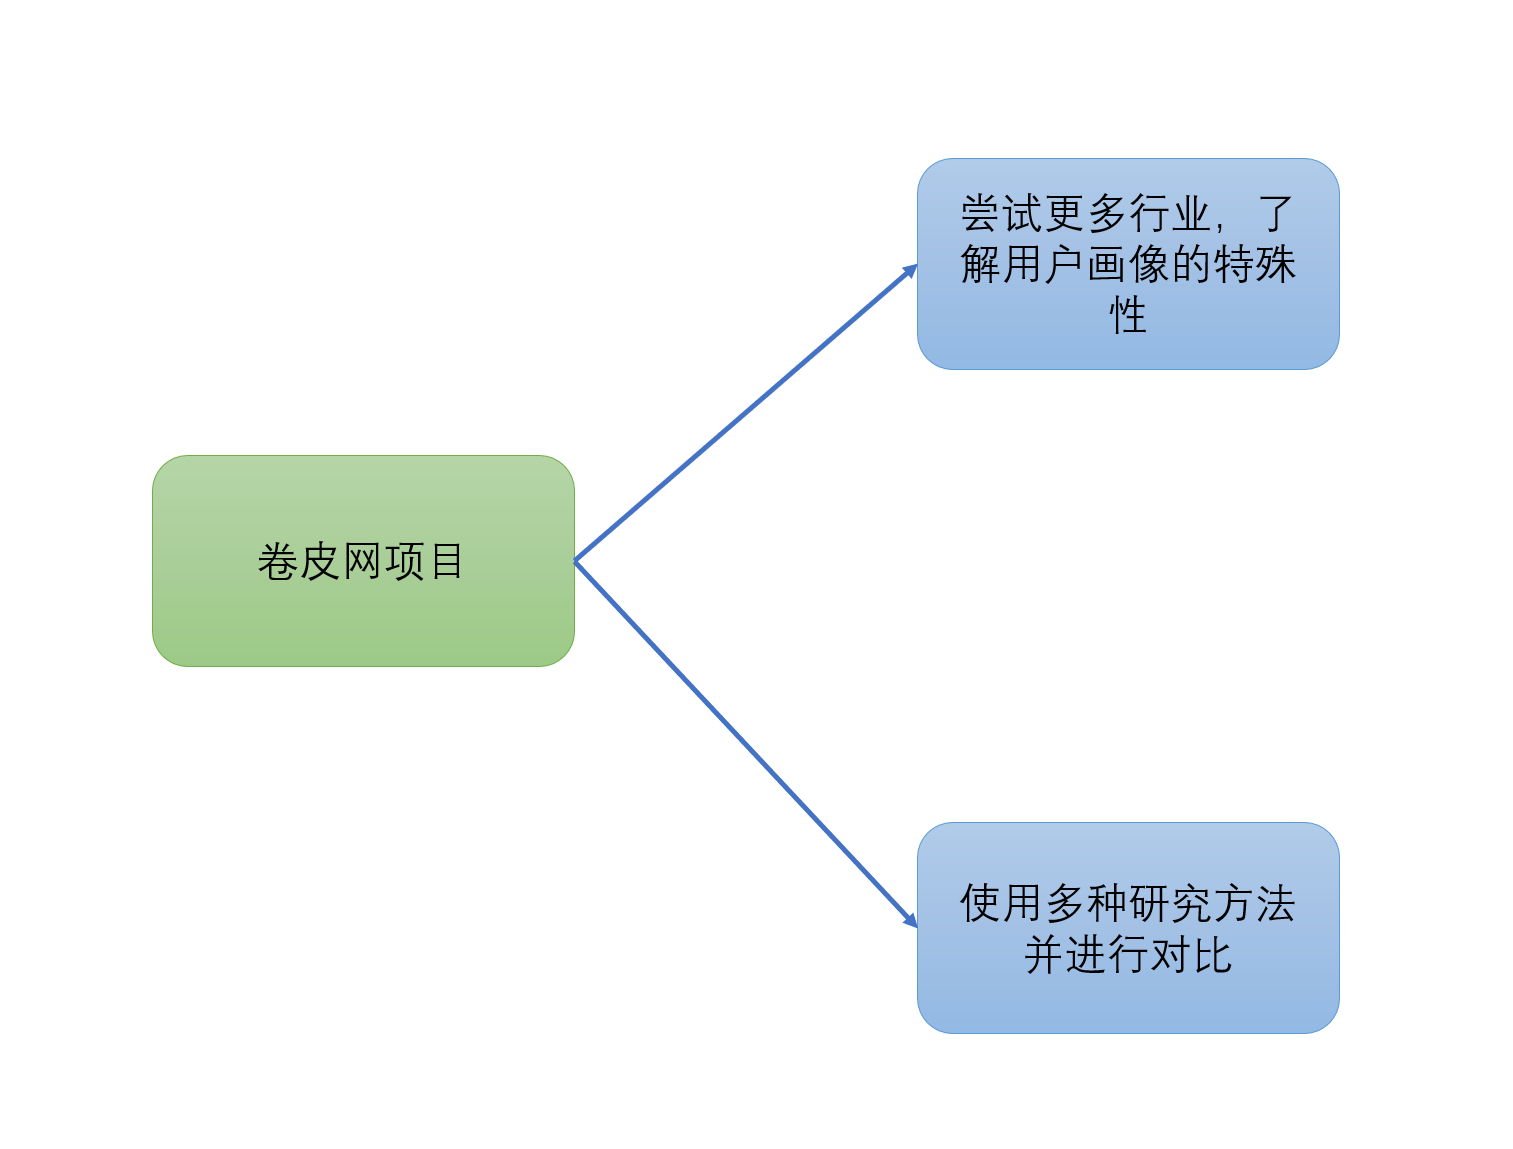
\includegraphics[height=0.7\paperheight]{amplify}
\end{frame}

\begin{frame}{工作范围扩大}
   \begin{itemize}
      \item 分析不同行业的数据和用户,全方位解读用户画像的企业应用场景。\newline
      \item 对比不同编程语言及程序包的优劣。\newline
      \item 通过建立网页版教程,系统归纳团队研究过程及心得,给入门用户提供学习的平台。\newline
      \item 编写入门级机器学习实践案例,增强教程的实践性与互动性。
   \end{itemize}
\end{frame}

\begin{frame}{为什么要做教程?}
  \begin{itemize}
    \item 在卷皮网项目开发过程中发现,相关技术资料不够系统,教程较少,推荐困难。\newline
    \item 身边许多老师同学对此领域有很浓厚的兴趣。
  \end{itemize}
\end{frame}

\begin{frame}{网页}
\begin{columns}
  \begin{column}{0.4\textwidth}
    \textbf{userprofileguide.github.io}
  \end{column}
  \begin{column}{0.6\textwidth}
    
\includegraphics[height=0.4\paperheight]{website1}
    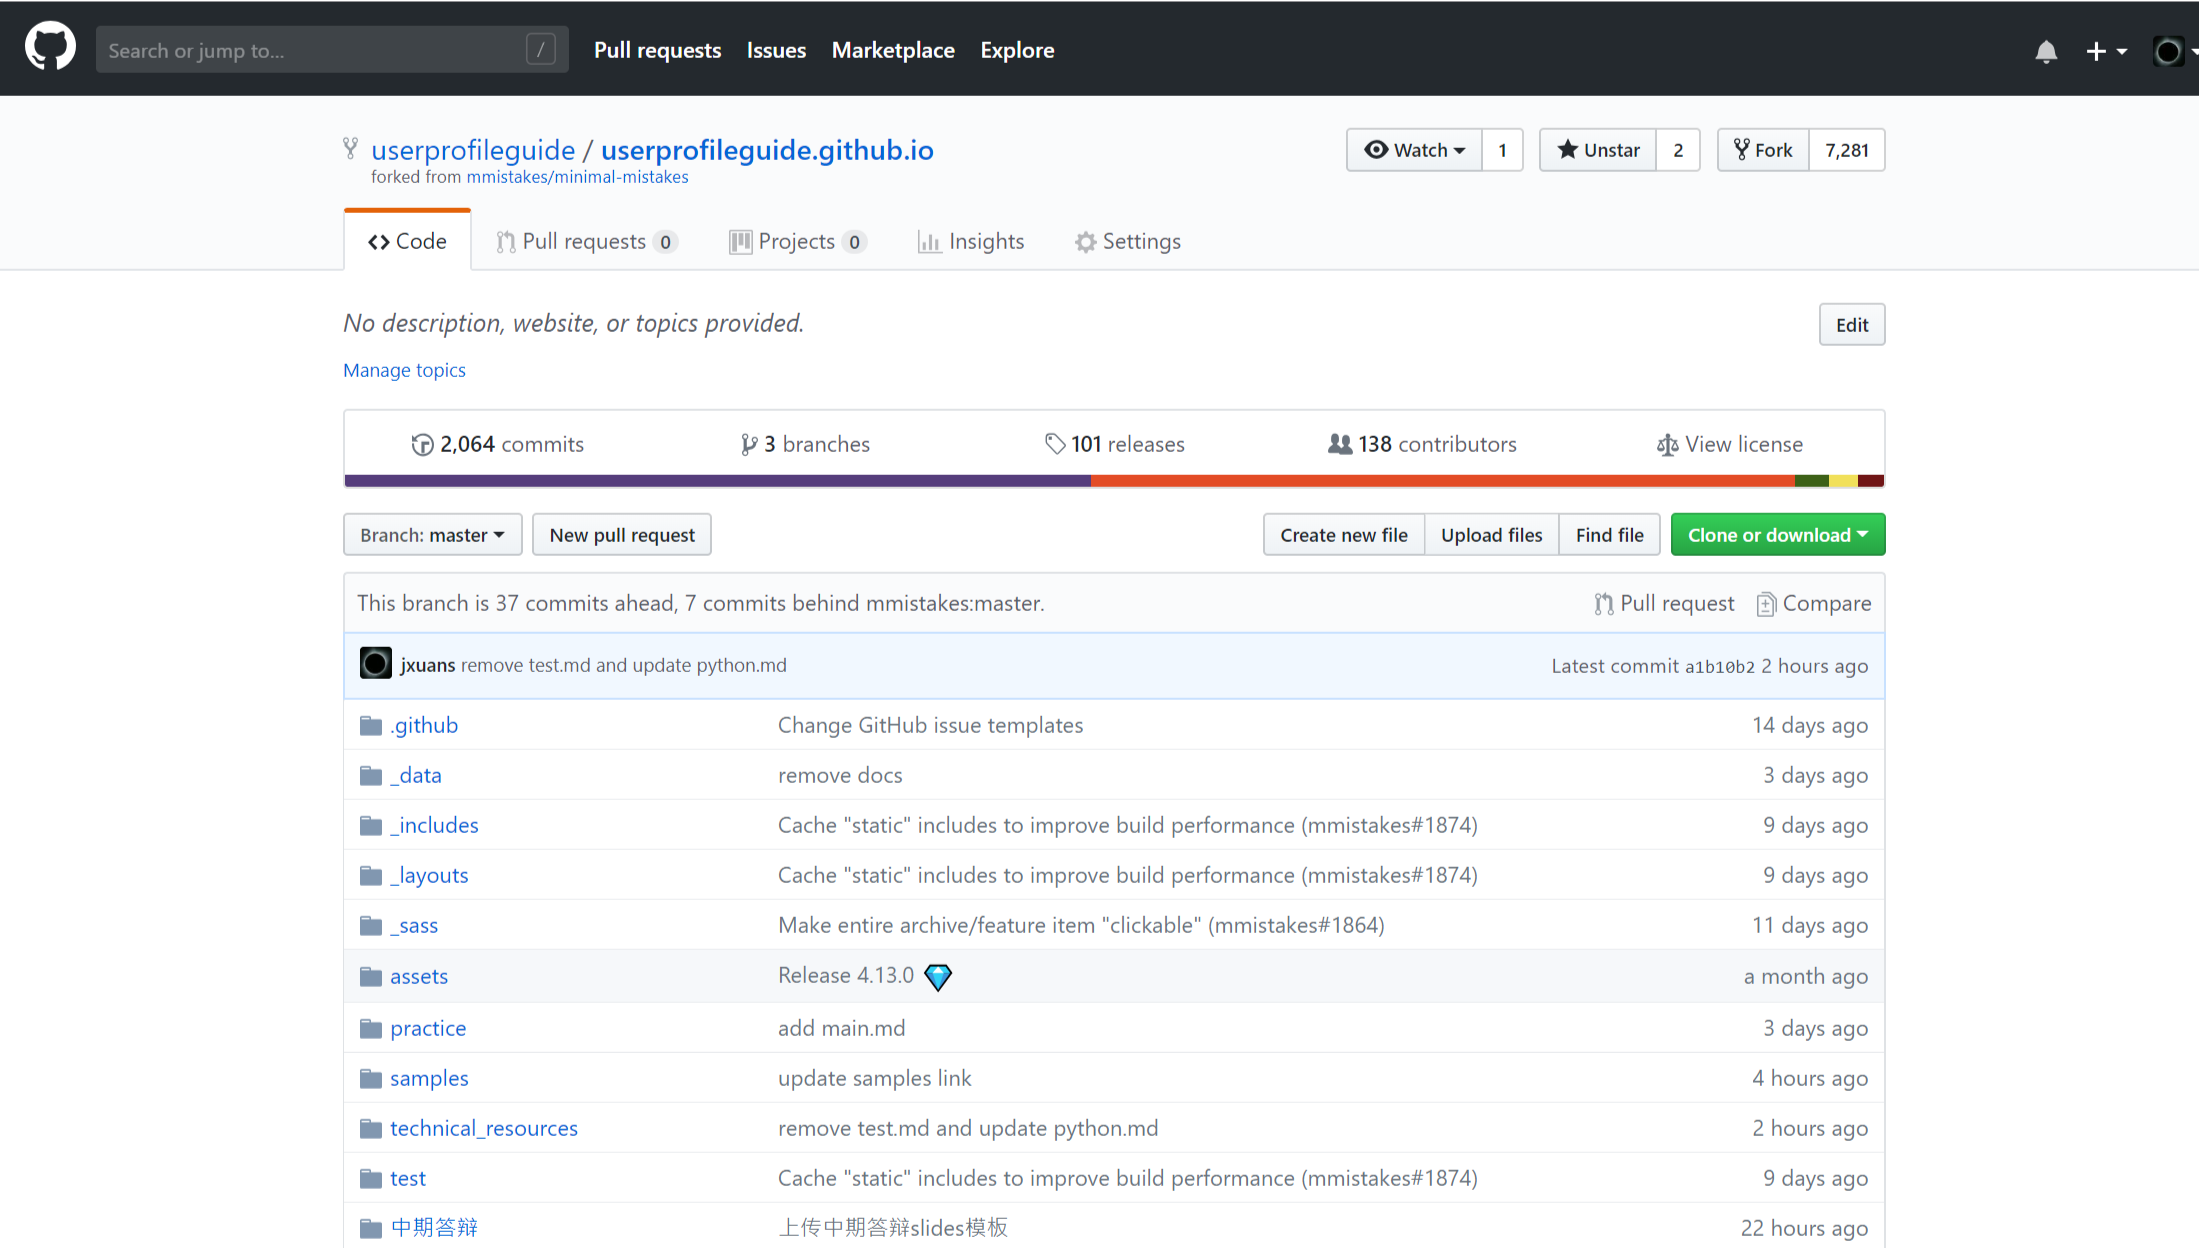
\includegraphics[height=0.4\paperheight]{website2}
  \end{column}
  \end{columns}
\end{frame}

\begin{frame}{教程框架设计}
\begin{itemize}
\item 技术原理:对概念和基础知识点的介绍、程序包的使用方法介绍、算法原理介绍等。\newline
\item 案例分析:全面记录团队项目开发过程和在其中使用到的研究方法、编程技巧、优化思路,并进行探讨比较。\newline
\item 入门练习:提供让入门读者快速上手实践并理解机器学习和用户画像的案例,数据与源代码。\newline
\end{itemize}
\end{frame}

\begin{frame}{已完成教程}
  \begin{itemize}
    \item Python编程语言基础教程\newline
    \item 机器学习简介\newline
    \item 用户画像简介及企业实例\newline
    \item 银行客户流失案例分析\newline
    \item R语言基础及机器学习入门\newline
  \end{itemize}
\end{frame}

\begin{frame}{即将上线教程}
  \begin{itemize}
    \item 卷皮网项目开发历程,数据,代码,总结\newline
    \item 机器学习主流论坛与资源获取站点\newline
    \item 如何使用GitHub进行项目开发\newline
    \item Kaggle的使用方法\newline
    \item Stack Overflow上有哪些有用的项目实战经验?\newline\newline
  \end{itemize}
  \textbf{以上教程将在一个月内上线}
\end{frame}
%%%%%%



\section{财务情况}
  \begin{frame}{财务情况}
  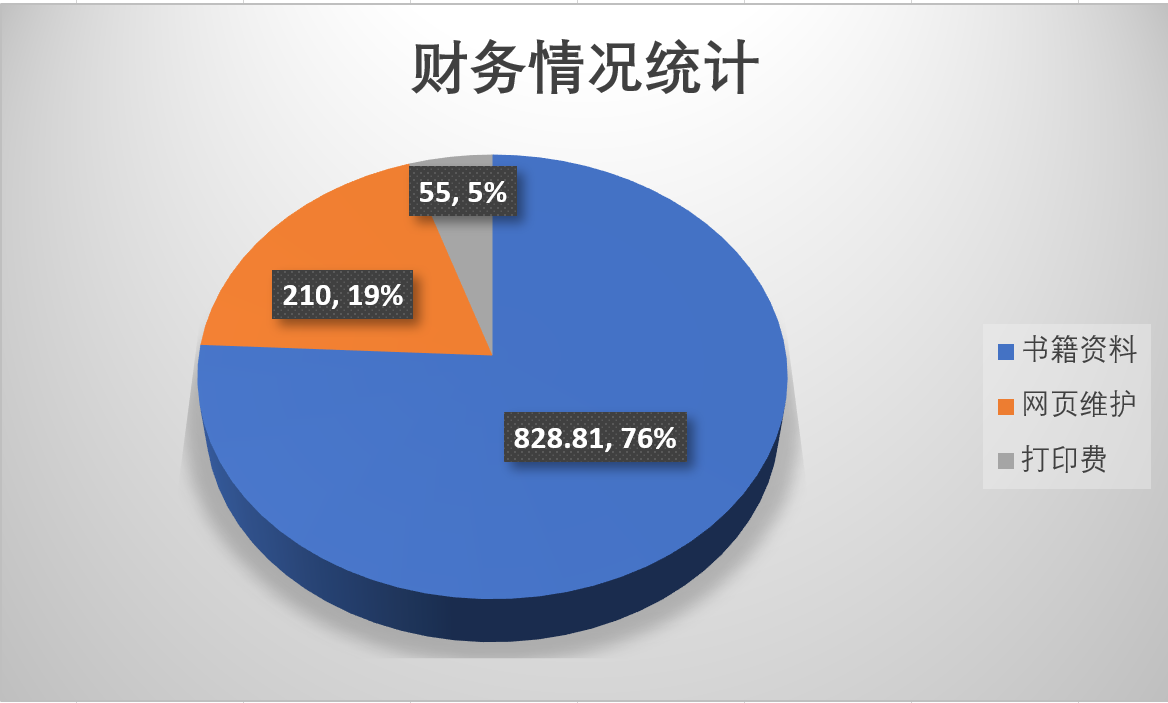
\includegraphics[height=0.66\paperheight]{finance}
  \end{frame}

%%%%%%

\section{后续工作安排}
\begin{frame}{后续工作安排}
  \begin{itemize}
    \item 拓宽研究领域,完成更多项目开发案例。\newline
    \item 继续完善教程主体部分和延申部分,增强内容的完整度与可读性。\newline
    \item 与企业进行合作,进一步探讨用户画像的商业价值与伦理学边界。\newline
    \item 扩大影响力,打造可持续发展编程社区,不断引入更多优质内容,吸引越来越多的同行加入。
  \end{itemize}

\end{frame}


%%%%%%


\end{document}
